        \maketitle
        \tableofcontents
		\section{Grundlagen}
		\subsection{Mathematik}
		\subsubsection{Mehrdimensionale Integrale}
		\begin{center}
			\textbf{Kurvenintegrale:}\\%
			\begin{align*}
				\int\limits_{\mathcal{C}}f(\vec{r})\mathrm{d}s &= \int\limits_a^b\ f(\vec{r}(t))\,|\vec{r^{\prime}}(t)|\mathrm{d}t;\
				\quad \vec{r}:[a,b]\to\mathcal{C}\\
				\int\limits_{\mathcal{C}}\vec{F}(\vec{r})\mathrm{d}s &= \int\limits_a^b\ \vec{F}(\vec{r}(t))\cdot\vec{r^{\prime}}(t)\mathrm{d}t;\
				\quad \vec{r}:[a,b]\to\mathcal{C}\\
			\end{align*}
			\textbf{Oberflächenintegrale:}
			\begin{align*}
				\iint\limits_A f \mathrm{d}\vec{a} &= \iint\limits_A f(\vec{x}(s,t))\!\
				\left\|\dfrac{\partial\vec{x}}{\partial s}\times\dfrac{\partial\vec{x}}{\partial t}\right\|\
				\mathrm{d}s\mathrm{d}t\\
				\iint\limits_A \vec{F} \mathrm{d}\vec{a} &= \iint\limits_A \vec{F}(\vec{x}(s,t))\cdot\!\
				\left( \dfrac{\partial\vec{x}}{\partial s}\times\dfrac{\partial\vec{x}}{\partial t} \right)\
				\!\mathrm{d}s\mathrm{d}t\\
			\end{align*}
			\textbf{Volumenintegrale:}
			\begin{align*}
				V &= \iiint\limits_V f(x,y,z)\:\mathrm{d}x\mathrm{d}y\mathrm{d}z\\
				&= \iiint\limits_V f(\rho,\varphi,z)\,\rho\:\mathrm{d}\rho\mathrm{d}\varphi\mathrm{d}z\\
				&= \iiint\limits_V f(r,\varphi,\theta)\,r^2\sin\theta\:\mathrm{d}r\mathrm{d}\varphi\mathrm{d}\theta\\
			\end{align*}
		\end{center}
        \subsubsection{Integraltheoreme}
        \textbf{Integralsatz von Gauß:}
            \[\iiint\limits_V \mathrm{div}\:\vec{a}\,\mathrm{d}v = \oiint\limits_{A(V)} \vec{a}\,\mathrm{d}\vec{A}\]
        \subsubsection{Vektoralgebra}
        %\(\vec{a}\times\vec{b} = -\vec{b}\times\vec{a}\)
        \textbf{Spatprodukt:}\\
        \[(\vec{a} \times \vec{b}) \cdot \vec{c} = (\vec{c} \times \vec{a}) \cdot \vec{b}\]\\
	 \subsection{Maxwell-Gleichungen}
	 \subsubsection{Integralform}
		{\small%
		\begin{flalign*}
			& \mathrm{\textbf{Gauß'sche Gesetz:}}\\
			& \oiint\limits_{A(V)}\vec{D}_m\cdot\mathrm{d}\vec{A} = \iiint\limits_V\rho\mathrm{d}V = Q\\
			& \mathrm{\textbf{Magnetische Quellenfreiheit:}}\\
			& \oiint\limits_{A(V)}\vec{b}\cdot\mathrm{d}\vec{A} = 0\\
			& \mathrm{\textbf{Induktionsgesetz:}}\\
			& \oint\limits_C\vec{e}\cdot\mathrm{d}\vec{s} =%
			-\dfrac{\mathrm{d}}{\mathrm{d}\vec{t}}\iint\limits_A\vec{b}\cdot\mathrm{d}\vec{A} = -\dfrac{\mathrm{d}\Phi_m}{\mathrm{d}t}\\
			& \mathrm{\textbf{Durchflutungsgesetz:}}\\
			& \oint\limits_C\vec{h}\cdot\mathrm{d}\vec{s} = \iint\limits_A\left[\vec{j}+\dfrac{\mathrm{d}\vec{D}_m}{\mathrm{d}t}\right]\cdot\mathrm{d}\vec{A} = i_{ges}\\
		\end{flalign*}
		}
	 \subsubsection{(Zeitfreie) Differentielle Form}
	 {\small%
	 \begin{align*}
	  &\mathrm{\textbf{Differentiell}} & \mathrm{\textbf{Zeitfrei (harm. Wellen)}}\\
	 	&\nabla\times\vec{e} = -\dfrac{\partial\vec{b}}{\vec{\partial t}} & \nabla\times\vec{E} = -j\omega\vec{B}\\
	 	&\nabla\times\vec{h} = \vec{j} +\dfrac{\partial\vec{D}_m}{\vec{\partial t}} & \nabla\times\vec{H} = \vec{J} + j\omega\vec{D}_m\\
		&\nabla\cdot\vec{D}_m = \rho & \nabla\cdot\vec{D}_m = \rho\\
		&\nabla\cdot\vec{b} = \rho_m & \nabla\cdot\vec{B} = \rho_m
	 \end{align*}
	 }
	 \subsubsection{Kontinuitätsgleichung des Stroms}
	 {\small%
	 \begin{align*}
	 	& \mathrm{\textbf{Integrale Form}}\\
		& \oint\limits_{A(V)}\vec{j}\cdot\mathrm{d}\vec{A} = -\int\limits_v \dfrac{\partial \rho}{\partial t} \mathrm{d}v\\
		& \mathrm{\textbf{Differentielle Form}}\\
		& \nabla\cdot\vec{j} = -\dfrac{\partial \rho}{\partial t}\\
		& \mathrm{\textbf{Zeitfreie Form}}\\
		& \nabla\cdot\vec{J} = -j\omega\rho
	 \end{align*}
	 \subsubsection{Entkopplung der Maxwell-Gleichungen}
	 \begin{itemize}
	 	\itemsep0pt
		\item Differentielle Maxwell-Gleichungen
		\item \(\epsilon_r, \mu_r = \mathrm{konst.}\)
		\item \(\kappa = 0, \vec{J} \neq 0\)\\
	 	\(\implies\) \textbf{Wellengleichung:}\\\vspace{2pt}
		\(\nabla\!\times\!\nabla\!\times\!\vec{E} - k^2\vec{E} = -j\omega\mu_r\mu_0\vec{J}\)
		\item Quellenfrei \(\vec{J} = 0\)
		\item \(\nabla\!\times\!\nabla\!\times\!\vec{F} = \mathrm{grad}\;\mathrm{div}\vec{F} - \Delta\vec{F}\)\\
		\(\implies\) \textbf{Helmholtz-Gleichung:} \(\Delta\vec{E} + k^2\vec{E} = 0\)
	 \end{itemize}

	 \subsubsection{Rand- und Stetigkeitsbedingungen}
	 \begin{itemize}
	 	\itemsep0pt
		\item \textbf{Tangentialkomponenten}
		\begin{itemize}
			\itemsep0pt
			\item Normalfall: \(\vec{n}\times\left(\vec{h}_1 - \vec{h}_2\right) = 0\)
			\item Oberflächenströme: \(\vec{n}\times\left(\vec{h}_1 - \vec{h}_2\right) = \vec{j}_F\)
			\item \(\vec{n}\times\left(\vec{e}_1 - \vec{e}_2\right) = 0\)
		\end{itemize}
		\item \textbf{Normalkomponenten}
		\begin{itemize}
			\itemsep0pt
			\item Normalfall: \(\vec{n}\cdot\left(\vec{D}_{m1} - \vec{D}_{m2}\right) = 0\)
			\item Oberflächenladungen: \(\vec{n}\cdot\left(\vec{D}_{m1} - \vec{D}_{m2}\right) = \rho_F\)
			\item \(\vec{n}\cdot\left(\vec{b}_1 - \vec{b}_2\right) = 0\)
		\end{itemize}
	 \end{itemize}
	 }

	 \subsection{Skin-Effekt}%
	 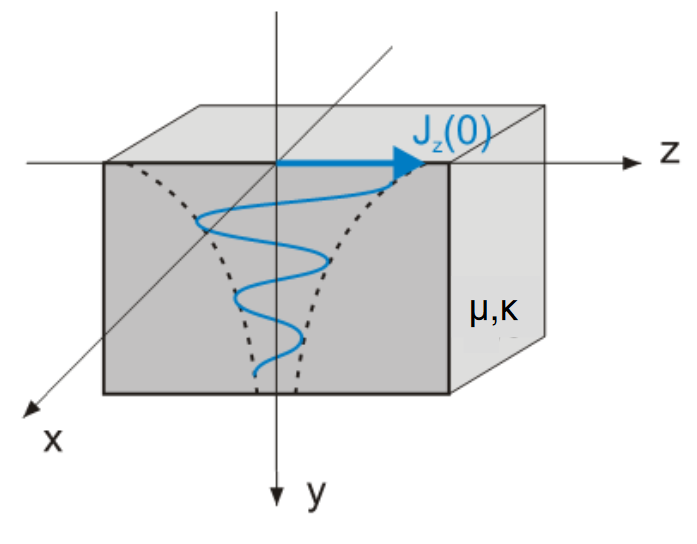
\includegraphics[width=.3\paperheight]{content/fuw/pictures/skin_effect.png}
	 {\small%
	 \begin{itemize}
	 	\itemsep0pt
		\item ideale Leiter \(\kappa\to\infty:\: E_{tan} = 0\)\\
		\(\implies\) nur in einer infitesimal dünnen Schicht existieren Oberflächenströme
		\item guter Leiter \(\kappa\gg\omega\epsilon\), verlustbehaftet:
		\begin{itemize}
			\itemsep0pt
			\item in einer dünnen Schicht unter der Oberfläche existieren nennenswerte Stromdichten\\
			\item Für die Verluste sind nur die obersten Schichten des Leiters entscheidend
			\item \textbf{Stromverteilung im Leiter:}\\
			\(J_z = J_z(0)e^{-ky}e^{-jky};\;\;k=\sqrt{\dfrac{\omega\mu\kappa}{2}}\)\\
			\(\implies \mathrm{\textbf{Eindringtiefe:}}\;\; \delta = \dfrac{1}{k} = \sqrt{\dfrac{2}{\omega\mu\kappa}}\)
		\end{itemize}
		\item Joule'sche Verluste: \(P_J = \frac{1}{2}\int\limits_S R_S |H_0|^2\mathrm{d}A\)\\
		\(\implies\) \textbf{Oberflächenimpedanz:}\\
		\(Z_S = R_S (1 + j) = (1 + j)\sqrt{\dfrac{\omega\mu}{2\kappa}}\)
	 \end{itemize}
	 }

	 \subsection{Ebene Wellen}
	 {\small%
	 \subsubsection{Ebene Wellen mit Ausbreitung in z-Richtung}
	 \begin{enumerate}
	 	\itemsep0pt
		\item Gute Approximation für reale Wellen \(\to\) Fernfelder von Antennen als lokal ebene Wellen
		\item Darstellung beliebiger Wellenfelder als Überlagerung ebener Wellen \(\to\) Fourier-Transformation
		\item Einfach handhabbar, z.B. bei Einfall auf ebene Grenzflächen
	 \end{enumerate}
	 \begin{itemize}
	 	\itemsep0pt
		\item Phasenfronten sind Ebenen
		\item Wellenvektor \(\vec{k}\) ist normal zu den Ebenen
		\item Ausbreitung in z-Richtung: \(\frac{\partial}{\partial x} = \frac{\partial}{\partial y} = 0\)
		\item (stückweise) homogenes, lineares Medium: \(\mu, \epsilon = \mathrm{const.}\)
		\item keine freie Ladungen: \(\rho = 0\)
		\item verschwindende Leitfähigkeit: \(\kappa = 0\)\\
		\(\implies\) Symmetrie, d.h. Lösung für E-Feld \textit{oder} H-Feld genügt
		\item ist eine \textbf{TEM-Welle} (nicht-dispersiv, keine longitudinale Komponente)
		\item 1D-Helmholtz-Gleichung: \(\dfrac{\partial^2e_x}{\partial z^2} - \epsilon\mu \dfrac{\partial^2 e_x}{\partial t^2} = 0\)\\
		\(\implies\) Lösung:\\
		\(e_x(z,t) = E_1 f_1\left(t - \dfrac{z}{c}\right) + E_2 f_2\left(t + \dfrac{z}{c}\right)\)\\
		\(\implies\) Ausbreitungsgeschwindigkeit: \(c = \dfrac{1}{\sqrt{\epsilon\mu}}\)
		\item \(e_x(z,t) = \sqrt{\dfrac{\mu}{\epsilon}} h_y(z,t) = Z_F\, h_y(z,t) \)\\
		\(\implies\) \textbf{Wellenwiderstand des Vakuums:}\\
		\(Z_{F_0} = \sqrt{\dfrac{\mu_0}{\epsilon_0}} \approx 120\pi\,\Omega \approx 377\,\Omega\)
	 \end{itemize}
	 \subsubsection{Harmonische Ebene Wellen}
	 \begin{flalign*}
	 	e_x(z,t) &= E \cos\left[\omega\left(t - \dfrac{z}{c}\right)\right]\\
		h_y(z,t) &= \dfrac{E}{Z_F} \cos\left[\omega\left(t - \dfrac{z}{c}\right)\right]
	 \end{flalign*}
	 \begin{itemize}
	 	\itemsep0pt
		\item Periodenabstand/Wellenlänge:\\
		\(\lambda = \dfrac{2\pi c}{\omega} = \dfrac{c}{f}\)
		\item \textbf{Phasenkonstante \(\beta\):}\\
		\(\beta = \dfrac{\omega}{c} = \dfrac{2\pi}{\lambda}\)
		\item zeitfreie Gleichungen:\\\smallskip
		\(E_x(z,t) = \mathrm{Re}\left\{E_x(z)e^{j\omega t}\right\}\)\\
		\(\implies E_x(z) = E e^{-j\beta z}\)\\
		\(\implies H_y(z) = \dfrac{E}{Z_F} e^{-j\beta z}\)
	 \end{itemize}
	 \subsubsection{Polarisation Ebener Wellen}
	 % TODO: Add screenshot with from Polarization slide
	 \subsubsection{Phasen-/Gruppengeschwindigkeit}
	 \begin{itemize}
	 	\itemsep0pt
		\item \textbf{Dispersionsfreiheit} \(\implies v_{ph} = \dfrac{\omega}{\beta} = v_g\)
		\item Wellenlänge (Phasengeschwindigkeit) frequenzabhängig \(\to\) Frequenzkomponenten eines Signals breiten sich unterschiedlich schnell aus
		\item die Ausbreitungsgeschwindigkeit der Modulation bezeichnet man als \textbf{Gruppengeschwindigkeit:}\\\smallskip
		\(v_g = \dfrac{1}{\Delta\beta / \Delta\omega} \;\implies v_g = \left(\dfrac{\mathrm{d}\beta}{\mathrm{d}\omega}\right)^{-1}\)
	 \end{itemize}
	 \subsubsection{Allgemeine Ebene Wellen}
	 \begin{itemize}
	 	\itemsep0pt
		\item Allgemeiner Ansatz:\\
		\(\vec{E} = \vec{E}_0\,e^{-j\vec{k}\cdot\vec{r}};\;\;\vec{H} = \vec{H}_0\,e^{-j\vec{k}\cdot\vec{r}}\)
		\item Wellenzahlvektor:\\
		\(\vec{k} = k_x\vec{e}_x + k_y\vec{e}_y + k_z\vec{e}_z\)
		\item Ortsvektor:\\
		\(\vec{r} = x\vec{e}_x + y\vec{e}_y + z\vec{e}_z\)
		\item \(\vec{k}\cdot\vec{k} = \beta^2 - \alpha^2 - j2\vec{\alpha}\cdot\vec{\beta} = \omega^2\epsilon\mu\)
	 \end{itemize}

 \subsection{Reflexion und Brechung}
 \begin{itemize}
     \itemsep0pt
     \item Brechungsgesetz von Snellius:\\
         \(n_1 \sin(\theta_1) = n_2 \sin(\theta_2)\)
     \item Fresnel-Koeffizienten ($\perp$):\\
         \begin{align*}
             \rho_\perp &= \dfrac{Z_{F2} \cos(\theta_1) - Z_{F1}\cos(\theta_2)}{Z_{F2}\cos(\theta_1) + Z_{F1} \cos(\theta_2)},\\
             \tau_\perp &= \dfrac{2Z_{F2} \cos(\theta_1)}{Z_{F2}\cos(\theta_1) + Z_{F1} \cos(\theta_2)}
         \end{align*}
     \item Fresnel-Koeffizienten ($\parallel$):\\
         \begin{align*}
             \rho_\parallel &= \dfrac{Z_{F1} \cos(\theta_1) - Z_{F2}\cos(\theta_2)}{Z_{F1}\cos(\theta_1) + Z_{F2} \cos(\theta_2)},\\
             \tau_\parallel &= \dfrac{2Z_{F2} \cos(\theta_1)}{Z_{F1}\cos(\theta_1) + Z_{F2} \cos(\theta_2)}
         \end{align*}

 \end{itemize}
 \subsection{Gauß'scher Strahl}
 \subsection{TEM-Leitungen}
 {\centering%
 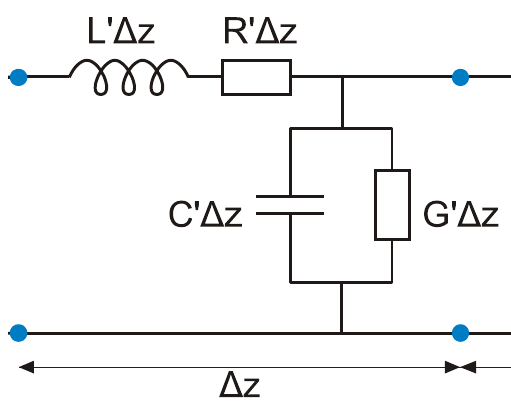
\includegraphics[width=.2\paperheight]{content/fuw/pictures/fuw_tem_ersatzschaltbild.png}
  \begin{itemize}
     \itemsep0pt
     \item \textit{quasi-TEM} (\(\beta = \sqrt{\epsilon_{r,\mathrm{eff}}} k_0 \neq \sqrt{\epsilon_r} k_0\))
     \item Kapazitätsbelag mit ($C^\prime$) und ohne ($C_a^\prime, \epsilon_r = 1$) Dielektrikum
     \item \(\beta = \sqrt{\dfrac{C^\prime}{C_a^\prime}} = \sqrt{\epsilon_{r,\mathrm{eff}}} k_0\)
     \item Impedanzbereich eingeschränkt; typ. \SI{20}{\Omega}-\SI{300}{\Omega}
     \item \textbf{Berechnung der Kapazitätsbeläge:} entweder numerisch oder analytisch mit konforme Abbildung
     \item Ausbreitungsgeschwindigkeit: \(c = \dfrac{1}{\sqrt{L^\prime C^\prime}}\)
     \item \textbf{VSWR} (\textit{Viz-war}) \(= \dfrac{V_{\mathrm{max}}}{V_{\mathrm{min}}} = \dfrac{1 + |\rho|}{1 - |\rho|}\)
     \item \( \mathrm{Mit}\; z = \dfrac{Z_L}{Z_0} \begin{cases} \rho = \frac{z-1}{z+1}\\ z = \frac{1+\rho}{1-\rho} \end{cases}\)
  \end{itemize}
  }
 \subsection{Planare Leitungen}
 \centering
 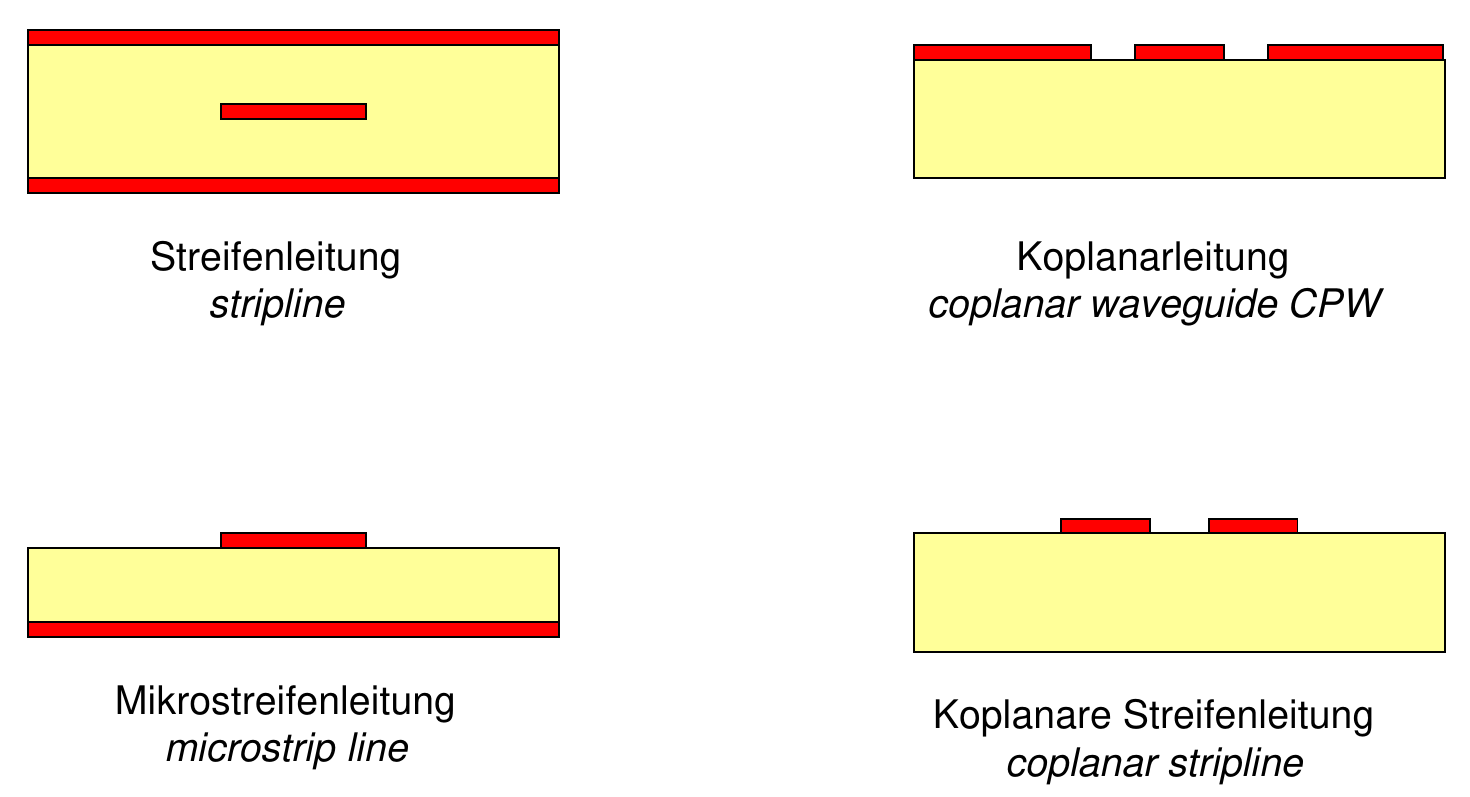
\includegraphics[width=.25\paperheight]{content/fuw/pictures/fuw_tem_leitungen.png}
 \begin{itemize}
     \itemsep0pt
     \item \textbf{Streifenleitung} $\implies$ echte TEM-Welle, \(\epsilon_r = \epsilon_{r,\mathrm{eff}}\)
     \item \textbf{Mikrostreifenleitung} $\implies$ einfache Fertigung, verlustarm, messtechnisch ungünstig
     \item \textbf{Koplanarleitung} $\implies$ messtechnisch günstig, serien-/parallelelemente leich integrierbar, mittlere Verluste, zwei Moden
     \item \textbf{Koplanare Streifenleitung}: symmetrisch, Leitungstranformer und Speiseleitung für Antennen 
 \end{itemize}
 }
